\section{Theory}
\markright{Theory}

A Zener diode is a specially doped silicon diode designed to operate in reverse breakdown without being damaged. Unlike an ordinary diode, which is mainly used in forward bias, the Zener diode is intentionally used in the reverse-bias region where the voltage reaches a specific value known as the Zener voltage, $V_Z$. At this point, the current rises sharply while the voltage across the diode remains nearly constant. This property makes it useful for voltage regulation and reference applications \cite{lab06_boylestad2013, lab06_mehta2012}.

In forward bias, a Zener diode behaves like a normal PN junction diode and begins to conduct once the applied voltage exceeds approximately $0.7\,\text{V}$ for silicon. In reverse bias, it allows only a small leakage current until the breakdown region is reached. Once the reverse voltage crosses the knee of the characteristic curve, the current increases rapidly without a significant change in the diode voltage. This nearly vertical region is the basis of voltage regulation, because the output voltage remains close to $V_Z$ even when the current varies over a wide range \cite{lab06_boylestad2013, lab06_manual2026}.

The Zener diode characteristic has three main regions: forward conduction, reverse leakage, and reverse breakdown. The complete I-V relationship is shown in Figure \ref{fig:lab06_iv_curve}. In the breakdown region, the voltage is almost constant, so the diode can be used as a stable reference source. That is why Zener diodes are commonly used in regulator circuits, clipping circuits, and protection networks \cite{lab06_mehta2012}.

\begin{figure}[H]
  \centering
  \begin{circuitikz}
    \draw (0,0) to[zD] (3,0);
  \end{circuitikz}
  \caption{Zener diode symbol.}
  \label{fig:lab06_symbol}
\end{figure}

Figure \ref{fig:lab06_symbol} shows the standard symbol of a Zener diode. It is similar to a normal diode symbol, but the cathode side is bent to indicate its reverse-breakdown operation. The actual device behavior is commonly explained using its I-V characteristic, which helps to identify the forward region, the leakage region, and the breakdown region.

\begin{figure}[H]
  \centering
  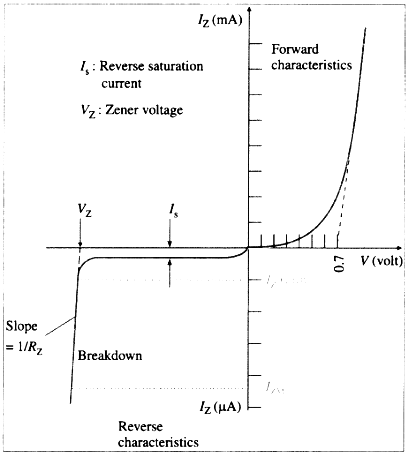
\includegraphics{lab-06/assets/i-v curve of a zener diode.png}
  \caption{I-V characteristic curve of a Zener diode \cite{lab06_sarthaks2026}.}
  \label{fig:lab06_iv_curve}
\end{figure}

A useful approximation for analysis is to treat the Zener diode as an ideal voltage source of value $V_Z$. This is called the first approximation, as shown in Figure \ref{fig:lab06_first_approx}. In this model, the voltage across the diode is assumed to remain constant whenever it is in the breakdown region, regardless of the current through it.

\begin{figure}[H]
  \centering
  \begin{circuitikz}
    % Zener diode
    \draw
    (0,0) node[ground] {}
    to[zD, l=$\text{Zener diode}$] (0,2)
    -- (0,3);

    % Equals sign
    \node at (2,1.5) {$=$};

    % Equivalent voltage source
    \draw
    (4,0) -- (4,1)
    to[battery1, invert, l_=$V_Z$] (4,2)
    -- (4,3);

    % + and - signs
    \node at (4.3,1.90) {$+$};
    \node at (4.3,1.20) {$-$};
  \end{circuitikz}
  \caption{First-approximation model of a Zener diode.}
  \label{fig:lab06_first_approx}
\end{figure}

A more realistic model is the second approximation, where the diode is represented as an ideal voltage source $V_Z$ in series with a small dynamic resistance $R_Z$, as shown in Figure \ref{fig:lab06_second_approx}. This additional resistance accounts for the slight change in voltage that occurs as current increases within the breakdown region. Since $R_Z$ is usually small, the output voltage remains close to the nominal Zener value and the device continues to behave as a practical voltage regulator \cite{lab06_manual2026}.

\begin{figure}[H]
  \centering
  \begin{circuitikz}
    % Zener diode
    \draw
    (0,0) -- (0,1)
    to[zD] (0,2)
    -- (0,3);

    % Equals sign
    \node at (1.5,1.5) {$=$};

    % Rz + Vz equivalent circuit
    \draw
    (3,3) -- (3,2.5)
    to[R, l_=$R_Z$] (3,1.5)
    -- (3,1)
    to[battery1] (3,0)
    -- (3,-0.5);

    % Voltage polarity and label
    \node at (3.35,0.90) {$+$};
    \node at (3.35,0.20) {$-$};
    \node at (3.8,0.5) {$V_Z$};
  \end{circuitikz}
  \caption{Second-approximation model of a Zener diode.}
  \label{fig:lab06_second_approx}
\end{figure}

This experiment is designed to study the forward and reverse characteristics of a Zener diode and to verify how it maintains a nearly constant voltage under varying current conditions.
